\section{Network Design Problems as Games}

In this section we establish the conceptual interpretation of network design problems as games.
Consider a road network in which link travel cost $\mathbf{t}$ is influenced not only by the link flow $\mathbf{x}$, but by control variables $\mathbf{y}\in Y$, where $Y$ represents a set of feasible control decisions.
In practice, the control variables could represent the cycle timing of traffic signals or the toll amount on a certain road segment.
A \textit{traffic controller} modulates the control variables $\mathbf{y}$ with the intent to keep traffic flow in some desirable set of states.
The \textit{vehicle fleet}, on the other hand, endeavors to \textit{individually} minimize their own travel time through the network, that is, satisfy the traffic network equilibrium.

\begin{figure}[!ht]
    \centering
    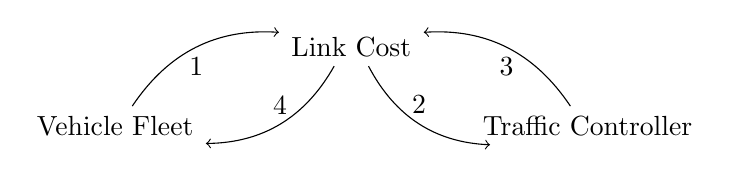
\begin{tikzpicture}
        \node (Y) at (6, 0) {Traffic Controller};
        \node (Z) at (0, 0) {Vehicle Fleet};
        \node (t) at (3, 1) {Link Cost};
        
        \draw[every loop]
            (Z) edge [bend left] node[below] {1} (t)
            (t) edge [bend left] node[above] {4} (Z)
            (Y) edge [bend right] node[below] {3} (t)
            (t) edge [bend right] node[above] {2} (Y)
        ;
    \end{tikzpicture}
    \caption{Influence of traffic controller and vehicle fleet choices on network state.}
    \label{fig:influence-diagram}
\end{figure}

We can conceptualize the cycle of influence between the traffic controller, the vehicle fleet, and the link travel cost with the following steps corresponding to the numbered arrows in \cref{fig:influence-diagram}.

\begin{enumerate}
    \item The vehicle fleet selects a traffic assignment $\mathbf{x}$ to fulfill the origin-destination demand $\mathbf{q}$ in such a way to minimize individual travel time.
    The network is now at traffic equilibrium.
    \item The traffic controller observes the link cost (or equivalently, the link flow).
    \item Using their observations of the network state and some control logic, the traffic controller chooses the control parameters $\mathbf{y}$.
    \item The vehicle fleet observes the (new) link cost function and uses it to inform their subsequent route choice.
\end{enumerate}

% What is the shared state space and how does it evolve?
% in other words, what is x'(s) = f(s, x(s), y(s), z(s))?
% what is s?

In the static traffic assignment problem, vehicles are assigned to all links that they will use on their route simultaneously. This is equivalent to the assumption that all vehicles start at the same time and 

\subsection{Formulation as a saddle point problem}

As presented in \citet{konnov2007equilibrium}, let $U\subseteq \mathbb{R}^l$ and $V\subseteq \mathbb{R}^m$ both be closed and convex sets. 
Let $L:\mathbb{R}^l\times\mathbb{R}^m \to \mathbb{R}$ be differentiable convex-concave, i.e., $L(\cdot, v)$ is convex for each $v\in V$ and $L(u, \cdot)$ is concave for each $u\in U$.
The \textit{saddle point problem} is to find a pair of points $u^*\in U$, $v^*\in V$ such that

\begin{align}
    L(u^*, v) \leq L(u^*, v^*) \leq L(u, v^*)\ \forall u \in U, v\in V
\end{align}

If we take $n=l+m$, $X= U\times V$, and define $G(x)=G(u, v) = \begin{bmatrix}\nabla_u L(u, v) & -\nabla_v L(u, v)\end{bmatrix}$, then the saddle point problem is equivalent the variational inequality $G(x^*)(x-x^*)\geq 0 \forall x\in X$.
